我们可以把函数$y(x)$看成一个运算符。对于任意输入$x$,这个运算符都能返回一个输出$y$。使用同样的方式,我们可以定义泛函(functional)$F[y]$是一个运算符,这个运算符以函数$y(x)$作为输入,返回输出$F$。泛函的一个例子是二维平面中的一条曲线的长度,这条曲线的轨迹要根据函数来定义。在机器学习领域,广泛使用的泛函是连续变量$x$的熵$H[x]$,因为对于任意概率密度函数$p(x)$的选择,它都返回一个标量值表示这个概率密度下$x$的熵。因此,$p(x)$的熵写成$H[p]$也一样没错。

传统的微积分中的一个常见的问题是找到一个$x$值使得$y(x)$取得最大值或者最小值。类似地,变分法中,我们寻找一个函数$y(x)$来最大化或者最小化泛函$F[y]$。即,对于所有可能的函数$y(x)$,我们想找到一个特定的函数,使得$F[y]$达到最大值或者最小值。变分法可以用来说明两点之间的最短路径是一条直线,或者最大熵分布是高斯分布。

按照微积分规则,我们在求传统的导数$\frac{\mathrm{d}y}{\mathrm{d}x}$时,我们可以首先让变量$x$产生一个小的改变$\epsilon$,然后对$\epsilon$进行幂级数展开,即
\begin{equation}
\label{tuiguang}
	y(x+\epsilon)=y(x)+\frac{\mathrm{d}y}{\mathrm{d}x}\epsilon+O(\epsilon^2)
\end{equation}
最后取极限$\epsilon\to 0$。类似地,对于一个多变量函数$y(x_1,\dots,x_D)$,对应的偏导数通过下式定义
\begin{equation}
	y(x_1+\epsilon_1,\dots,x_D+\epsilon_D)=y(x_1,\dots,x_D)+\sum_{i=1}^{D}\frac{\partial y}{\partial x_i}\epsilon_i +O(\epsilon^2)
\end{equation}
类似地,我们可以得到泛函的导数的定义。当我们对函数$y(x)$做一个微小的改变$\epsilon\eta(x)$(其中$\eta(x)$是$x$的一个信息任意的函数)时,我们考虑泛函$F[y]$的变化,如图所示
\begin{center}
	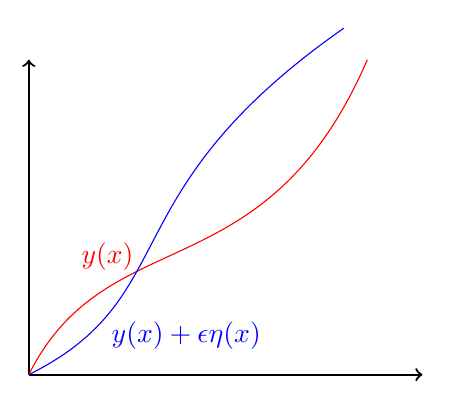
\begin{tikzpicture}
		\draw[->,thick] (0,0) -- (5,0);
		\draw[->,thick] (0,0) -- (0,4);
		
		\draw[red] (0,0) .. controls (1,2) and (3,1)  ..(4.3,4) node at (1,1.5){$y(x)$};
		\draw[blue] (0,0) .. controls (2,1) and (1,2.3).. (4,4.4) node at (2,0.5){$y(x)+\epsilon\eta(x)$};
	\end{tikzpicture}
\end{center}
我们把泛函$F[y]$关于$y(x)$的导数记作$\frac{\delta F}{\delta y(x)}$,通过下面的关系定义
\begin{equation}
\label{zhuanhua}
	F[y(x)+\epsilon\eta(x)]=F[y(x)]+\epsilon\int \frac{\delta F}{\delta y(x)}\eta(x) dx + O(\epsilon^2)
\end{equation}
这可以被看成公式$\ref{tuiguang}$的一个自然推广,其中$F[y]$现在依赖于变量的一个连续集合,即在所有$x$处的$y$值。令泛函的值在函数$y(x)$发生微小改变时几乎不变,可得
\begin{equation}
	\int \frac{\delta F}{\delta y(x)}\eta(x) dx=0
\end{equation}
由于这必须对任意的$\eta(x)$都成立,因此我们必须令泛函的导数等于零。为了证明这一点,让我们假设选择一个扰动$\eta(x)$,这个扰动只在点$\hat{x}$的邻域内等于零,在其他各处均不等于零。这种情况下,泛函的导数必须在$x=\hat{x}$处等于零。但是,由于这个结论必须对于任意的$\hat{x}$f都成立,因此泛函的导数必须对所有的$x$值都等于零。

考虑一个泛函,这个泛函由函数$G(y,y^{'},x)$的积分定义。函数$G(y,y^{'},x)$既依赖于$y(x)$又依赖于它的导数$y^{'}(x)$,还直接依赖于$x$。因此,这个泛函的形式为
\begin{equation}
	F[y]=\int G(y(x),y^{'}(x),x)dx
\end{equation}
其中,我们假设$y(x)$的值在积分边界(可能是无穷)处是定值。如果我们考虑函数$y(x)$的改变,那么我们有
\begin{equation}
	F[y(x)+\epsilon\eta(x)]=F[y(x)]+\epsilon\int \left\{\frac{\partial G}{\partial y}\eta(x)+\frac{\partial G}{\partial y^{'}}\eta^{'}(x) \right\}dx +O(\epsilon^2)
\end{equation}
我们现在必须把它转化为公式$\ref{zhuanhua}$的形式。为了完成这一点,我们将第二项进行分部积分,然后使用$\eta(x)$必须在积分边界处等于零的事实(因为$y(x)$在边界处为定值)。因此
\begin{equation}
		F[y(x)+\epsilon\eta(x)]=F[y(x)]+\epsilon\int \left\{\frac{\partial G}{\partial y}-\frac{d}{dx }\left(\frac{\partial G}{\partial y^{'}} \right) \right\}\eta(x)dx +O(\epsilon^2)
\end{equation}
我们可以直接读出泛函的导数。令泛函的导数等于零,我们有
\begin{equation}
	\frac{\partial G}{\partial y} - \frac{d}{dx}\left(\frac{\partial G}{\partial y^{'}} \right)=0
\end{equation}
这被称为欧拉-拉格朗日方程(Euler-Lagrange equation)。例如,如果
\begin{equation}
	G=y(x)^2+(y^{'}(x))^2
\end{equation}
那么,欧拉-拉格朗日方程的形式为
\begin{equation}
	y(x)-\frac{d^2y}{dx^2}=0
\end{equation}
使用$y(x)$的边界条件,我们可以解出这个关于$y(x)$的二阶微分方程。

通常情况下,我们考虑定义在积分上的泛函时,被积函数的形式为$G(y,x)$,不依赖于$y(x)$的导数。这种情况下,驻点只需要令$\frac{\partial G}{\partial y(x)}=0$对于所有的$x$都成立即可。

如果我们关于概率分布对泛函进行优化,那么我们需要保持概率的归一化限制。使用拉格朗日乘数法来进行优化是最方便的。使用拉格朗日乘数法之后,我们就可以进行无限制条件的最优化。

上述结果在多维变量$\boldsymbol{x}$上的扩展是很直接的。